% !Mode:: "Tex:UTF-8"
\chapter{面向流水线的对偶综合}
\label{chap:5}

\section{引言}
在通讯和多媒体芯片设计项目中,
最困难的一个工作是针对特定的协议,
如以太网\cite{IEEE8023_S4} 和PCI Express \cite{pcie21},
设计相应的编码器和解码器.
其中编码器负责将输入$\vec{i}$ 映射至输出$\vec{o}$,
而解码器则负责从$\vec{o}$中恢复$\vec{i}$。
对偶综合\cite{ShenICCAD09,ShenTCAD11,ShenTCAD12,LiuICCAD11,LiuTCAD12,TuDAC13}
假设$\vec{i}$ 总能够被$\vec{o}$的一个有限序列唯一决定,
以自动产生相应的解码器。
其中,
解码器的布尔函数可以使用Jiang et al. \cite{InterpBoolFunction}提出的算法,
该算法基于Craig插值\cite{Craig}。

通过研究现有的工业界编码器,我们发现他们都含有流水线结构以提高运行频率。
\begin{figure}[t]
\begin{center}
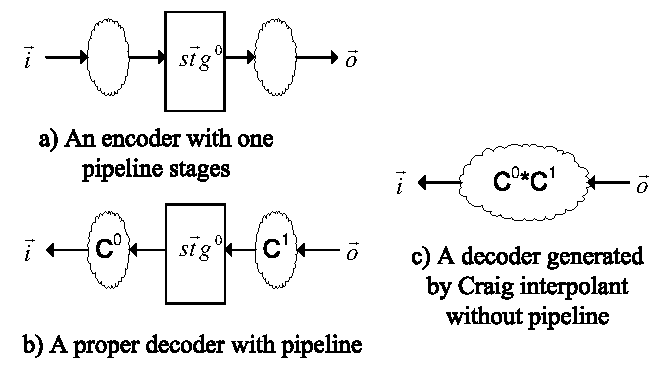
\includegraphics[width=0.5\textwidth]{pipeline_pipeline}
\end{center}
  \label{fig_pipe}
\caption{带有流水线的编码器和解码器}
\end{figure}

一个带有流水线的简单编码器如图\ref{fig_pipe}a)所示。
他的第一级流水线$\vec{stg}^0$ 包含数个寄存器。
其中输入变量$\vec{i}$ 被用于计算该级流水线$\vec{stg}^0$,
而流水线$\vec{stg}^0$ 则被用于计算$\vec{o}$。
根据该结构,
$\vec{stg}^0$ 能够被$\vec{o}$唯一决定,
而$\vec{i}$ 能够被$\vec{stg}^0$唯一决定。

因此,
一个由人类程序员设计的合理解码器,
应当如图\ref{fig_pipe}b)所示,
从$\vec{o}$ 中使用组合逻辑$C^1$恢复$\vec{stg}^0$ ,
并进一步使用组合逻辑$C^0$从$\vec{stg}^0$ 中恢复$\vec{i}$ 。
在此类解码器中,
关键路径被流水线级$\vec{stg}^0$切断,
以改善时序。



然而,
目前所有的对偶综合算法\cite{ShenTCAD11,ShenTCAD12,LiuICCAD11,LiuTCAD12,TuDAC13}
均使用Jiang提出的基于\cite{Craig}的算法 \cite{InterpBoolFunction}。
如图\ref{fig_pipe}c)所示,
这些算法从$\vec{o}$中使用一个大型组合逻辑$C^0*C^1$直接恢复$\vec{i}$,
这使得他们变得不必要的很慢,因为没有流水线寄存器切断这段复杂逻辑。

为了产生如图\ref{fig_pipe}b) 所示的解码器,
本文提出了一个新颖的算法。首先找到编码器中每一个流水线级$\vec{stg}^j$中的寄存器,
然后特征化每一个流水线级$\vec{stg}^j$的布尔函数,
已从下一个流水线级$\vec{stg}^{j+1}$ 或输出$\vec{o}$之中恢复$\vec{stg}^j$。
最终特征化$\vec{i}$的布尔函数以葱
第一个流水线级$\vec{stg}^0$中恢复$\vec{i}$。

\begin{figure}[t]
\begin{center}
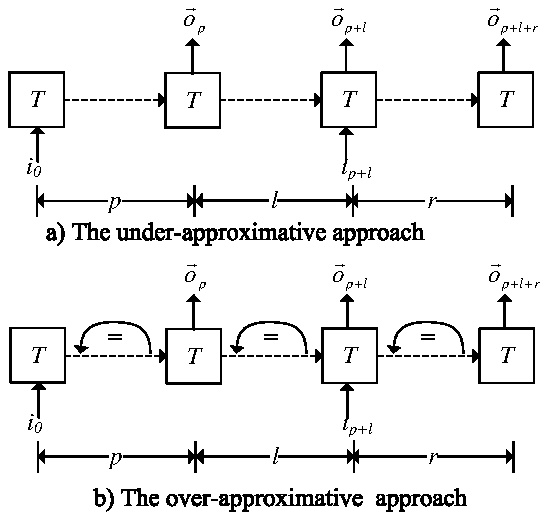
\includegraphics[width=0.5\textwidth]{pcln_pipeline}
\end{center}
\caption{下估计和上估计算法}
  \label{fig_pc}
\end{figure}

在复杂的工业界实际编码器,
如PCI Express \cite{pcie21} 和以太网\cite{IEEE8023_S4},
上的实验表明,
该算法总能够产生带有流水线级的快速解码器。.


\emph{本文剩余的内容安排如下}.
%Section \ref{sec_casestudy} explains our ideas with a simple example.
第\ref{sec_prem} 节介绍了背景知识;
第\ref{sec_pipeinfer} 节推导流水线结构,
而第\ref{sec_char} 节特征化每一个流水线级和输入的布尔函数;
第\ref{sec_exp} 和\ref{sec_relwork} 节给出实验结果和相关工作;
最后,
第\ref{sec_conclude} 节给出结论。



\section{背景知识}\label{sec_prem}

% \subsection{Flow control mechanism}\label{subsec_fc}



\subsection{命题逻辑可满足}\label{subsec_SAT}
布尔集合为$\mathbb{B}=\{0,1\}$。
变量向量表示为$\vec{v}=(v,\dots)$。
向量$\vec{v}$ 中的变量个数表示为$|\vec{v}|$。
若一个变量$v$ 是$\vec{v}$的成员,
则记为$v\in\vec{v}$;
否则$v\notin\vec{v}$.
$v\cup\vec{v}$ 是包含$v$ 和$\vec{v}$的所有成员的新向量。
$\vec{v}/\vec{w}$ 是一个包含$\vec{v}$ 的所有成员但是不包含$\vec{w}$的任意成员的新向量。
$\vec{a}\cup\vec{b}$ 是包含$\vec{a}$ 和$\vec{b}$的所有成员的新向量。
$\vec{v}$ 的赋值集合记为$[\![\vec{v}]\!]$,
比如,
$[\![(v_1,v_2)]\!]=\{(0,0),(0,1),(1,0),(1,1)\}$。


对于变量集合$V$上的公式$F$,
起命题逻辑可满足(SAT)  问题是指
如何找到$V$的一个赋值函数$A:V\to \mathbb{B}$,
使得$F$ 能够被赋值为$1$。
若$A$ 存在,则$F$ 是可满足的;
否则,
是不可满足的。

对于公式$\phi_A$ 和$\phi_B$,
若$\phi_A\wedge \phi_B$ 不可满足,
则存在公式$\phi_I$ 仅包含$\phi_A$ 和$\phi_B$ 的共同变量,
并使得$\phi_A\Rightarrow \phi_I$
且$\phi_I\wedge \phi_B$ 不可满足。
$\phi_I$ 称为$\phi_A$ 相对于$\phi_B$的Craig插值\cite{Craig}。
$\phi_I$ 可以使用McMillan提出的算法\cite{interp_McMillan}进行计算,
并应用于从一个布尔关系特征化出一个布尔函数\cite{InterpBoolFunction}。



\subsection{游有限状态机}\label{subsec_fsm}


编码器使用有限状态机模型(FSM) $M=(\vec{s},\vec{i},\vec{o},T)$,
其中$\vec{s}$为状态变量向量,
$\vec{i}$为输入变量向量,
$\vec{o}$为输出变量向量,
$T: [\![\vec{s}]\!]\times [\![\vec{i}]\!]\to [\![\vec{s}]\!]\times [\![\vec{o}]\!]$
是一个状态迁移函数,
用于从当前状态和输入变量向量,
计算出下一状态和输出变量向量。

$M$的行为可以通过展开迁移关系进行推导。
在第$n$步的$s\in\vec{s}$,$i\in\vec{i}$ 和$o\in\vec{o}$
分别表示为$s_n$, $i_n$ 和$o_n$。
另外,
在第$n$步的单个状态,输入和输出变量分别表示为$\vec{s}_n$,$\vec{i}_n$ 和$\vec{o}_n$。
一个路径是指$<\vec{s}_n,\dots,\vec{s}_m>$,
其中对于$n\le j< m$,
有$\exists \vec{i}_j\vec{o}_j (\vec{s}_{j+1},\vec{o}_j)\equiv T(\vec{s}_j,\vec{i}_j)$ 。
一个环是一个路径$<\vec{s}_n,\dots,\vec{s}_m>$ 满足$\vec{s}_n\equiv \vec{s}_m$。

\subsection{用于确定一个输入变量能否被输出向量的有限序列唯一决定的停机算法}\label{subsec_chkextdec}

该算法\cite{ShenTCAD11} 迭代的展开迁移函数。
对于每次迭代,
其分别调用一个下估计和一个上估计算法已给出确定的答案。
这两个算法分别在\ref{subsub_sound} 和\ref{subsub_complete}中给出。
我们酱紫啊\ref{subsub_algo} 中指出
这两者将最终收敛。

\subsubsection{下估计算法}\label{subsub_sound}

如图\ref{fig_pc}a)所示,
在展开的迁移函数序列上,
输入变量$i\in\vec{i}$ 能够被唯一决定的充分条件是,
存在$p$,$l$ 和$r$,
使得对于输出向量序列$<\vec{o}_p,\dots,\vec{o}_{p+l+r}>$的任意值,
$i_{p+l}$不能同时为0和1。
折等价于公式(\ref{uniqt1})中定义的$F_{PC}(p,l,r)$ 的不可满足性。

\begin{multline}\label{uniqt1}
% \begin{split}
F_{PC}(p,l,r):=\\
\left\{
\begin{array}{cc}
&\bigwedge_{m=0}^{p+l+r}
\{
(\vec{s}_{m+1},\vec{o}_m)\equiv T(\vec{s}_m,\vec{i}_m)
\}
\\
\wedge&\bigwedge_{m=0}^{p+l+r}
\{
(\vec{s'}_{m+1},\vec{o'}_m)\equiv T(\vec{s'}_m,\vec{i'}_m)
\}
\\
\wedge&\bigwedge_{m=p}^{p+l+r}\vec{o}_m\equiv \vec{o'}_m \\
\wedge& i_{p+l}\equiv 1 \wedge  i'_{p+l}\equiv 0
% \wedge&\bigwedge_{m=0}^{p+l+r}assertion(\vec{i}_m) \\
% \wedge&\bigwedge_{m=0}^{p+l+r}assertion(\vec{i'}_m)
\end{array}
\right\}
% \end{split}
\end{multline}



其中,
$p$ 是前置状态序列的长度,
$l$ 和$r$是两个用于唯一决定输入$i_{p+l}$的输出变量序列
$<\vec{o}_{p+1},\dots,\vec{o}_{p+l}>$ 和$<\vec{o}_{p+l+1},\dots,\vec{o}_{p+l+r}>$
的长度。
行2对应于图\ref{fig_pc}a)中的路径,
行3 是他的一个拷贝。
他们的长度是一样的。
行4 强制两者的输出序列具有相同的赋值,
而行5 强制他们的输入$i_{p+l}$ 不同。

根据公式(\ref{uniqt1}),
对于 $p'\ge p$, $l'\ge l$ 和$r'\ge r$,
$F_{PC}(p',l',r')$ 的短句集合是$F_{PC}(p,l,r)$的超集。
因此,
$F_{PC}(p,l,r)$的不可满足性
可以扩展到任意更大的$p'\ge p$, $l'\ge l$ 和$r'\ge r$。


\begin{proposition}\label{prop_pc1}
若$F_{PC}(p,l,r)$ 不可满足,
则对任意更大的$p$, $l$ 和$r$,
$i_{p+l}$ 可以被$<\vec{o}_{p},\dots,\vec{o}_{p+l+r}>$ 唯一决定。
\end{proposition}


\subsubsection{上估计算法}\label{subsub_complete}

若上一节定义的$F_{PC}(p,l,r)$ 可满足,
则存在两种可能性:
\begin{enumerate}
 \item
$i_{p+l}$ 可以在更大的$p$, $l$ 和$r$时,
被$<\vec{o}_{p},\dots,\vec{o}_{p+l+r}>$ 唯一决定;
 \item
$i_{p+l}$ 不能被任何$p$, $l$ 和$r$情况下的$<\vec{o}_{p},\dots,\vec{o}_{p+l+r}>$ 唯一决定。
\end{enumerate}

如果是第一种情况,
则通过迭代的增大$p$, $l$ 和$r$,
$F_{PC}(p,l,r)$ 总能够变成不可满足。
而如果是第二种情况,
则该算法不停机。



\begin{algorithm}[t]
\begin{algorithmic}[1]
\STATE{输入 :输入变量$i\in\vec{i}$.}
\STATE{输出: $i\in\vec{i}$ 是否能够被$\vec{o}$唯一决定,$p$, $l$ 和$r$的取值}
\STATE $p$:= 0; ~$l$:= 0;~$r$:= 0\;
\WHILE {$1$}
\STATE   $p$++;~$l$++;~$r$++\;\label{linepc1}
   \IF{$F_{PC}(p,l,r)$ 不可满足}
    \RETURN (yes, $p$, $l$, $r$);
   \label{lnsat}\ELSIF{$F_{LN}(p,l,r)$ 可满足}
    \RETURN (no, $p$, $l$, $r$);
   \ENDIF
\ENDWHILE
\caption{$CheckUniqueness(i)$: 检查
$i\in\vec{i}$ 能否被$\vec{o}$唯一决定的停机算法}
\label{alg_pcln}
\end{algorithmic}
\end{algorithm}



因此,
为了得到停机算法
我们需要区分上述两种情形。
该方法如图\ref{fig_pc}b)所示,
该图类似于图\ref{fig_pc}a),
不过增加了三个新的约束用于检测在$<\vec{s}_{0},\dots,\vec{s}_{p}>$,$<\vec{s}_{p+1},\dots,\vec{s}_{p+l}>$ 和
$<\vec{s}_{p+l+1},\dots,\vec{s}_{p+l+r}>$上的环。
其形式化的定义如公式(\ref{uniqln})
其中最后三行对应于新增加的三个环检测约束。

\begin{multline}\label{uniqln}
% \begin{split}
F_{LN}(p,l,r):=\\
\left\{
\begin{array}{cc}
&F_{PC}(p,l,r)\\
\wedge&\bigvee_{x=0}^{p-1}\bigvee_{y=x+1}^{p} \{\vec{s}_x\equiv \vec{s}_y\wedge \vec{s'}_x\equiv \vec{s'}_y\} \\
\wedge&\bigvee_{x=p+1}^{p+l-1}\bigvee_{y=x+1}^{p+l} \{\vec{s}_x\equiv \vec{s}_y\wedge \vec{s'}_x\equiv \vec{s'}_y\} \\
\wedge&\bigvee_{x=p+l+1}^{p+l+r-1}\bigvee_{y=x+1}^{p+l+r} \{\vec{s}_x\equiv \vec{s}_y\wedge \vec{s'}_x\equiv \vec{s'}_y\}
\end{array}
\right\}
% \end{split}
\end{multline}



当$F_{LN}(p,l,r)$ 可满足时,
则$i_{p+l}$ 不能被$<\vec{o}_{p},\dots,\vec{o}_{p+l+r}>$唯一决定。
更重要的是,
通过展开这三个环
我们可以把$F_{LN}(p,l,r)$ 的可满足性推广到更大的$p$, $l$ 和$r$上。
这意味着:


\begin{proposition}\label{prop_ln1}
如果$F_{LN}(p,l,r)$ 可满足,
则$i_{p+l}$ 对于任意更大的$p$, $l$ 和$r$,
不能被$<\vec{o}_{p},\dots,\vec{o}_{p+l+r}>$ 唯一决定。
\end{proposition}

其正确性证明的细节见\cite{ShenTCAD11}。

\subsubsection{完全算法}\label{subsub_algo}

基于Propositions \ref{prop_pc1} 和\ref{prop_ln1},
我们有如下算法\ref{alg_pcln}。
该算法搜索$p$, $l$ 和$r$ 使得
输入变量$i_{p+l}$ 能够被$<\vec{o}_{p},\dots,\vec{o}_{p+l+r}>$唯一决定。
\begin{enumerate}
 \item
一方面,
如果存在这样的$p$, $l$ 和$r$,
则令$p':=max(p,l,r)$, $l':=max(p,l,r)$ 和$r':=max(p,l,r)$。
从Propositions \ref{prop_pc1},
我们知道$F_{PC}(p',l',r')$ 不可满足。
因此$F_{PC}(p,l,r)$ 总能在行\ref{linepc1}称为不可满足;
 \item
另一方面,
如果不存在$p$, $l$ 和$r$,
则$p$, $l$ 和$r$ 总会变得比最长的无环路径更长,
这意味着在$<\vec{s}_{0},\dots,\vec{s}_{p}>$,$<\vec{s}_{p+1},\dots,\vec{s}_{p+l}>$ 和
$<\vec{s}_{p+l+1},\dots,\vec{s}_{p+l+r}>$上存在环。
这将使得$F_{LN}(p,l,r)$ 在行\ref{lnsat}变得可满足。
\end{enumerate}

两种情况都将导致上述算法停机。
其正确性和停机性证明的细节见\cite{ShenTCAD11} 。



\section{推导编码器的流水线结构}\label{sec_pipeinfer}

\subsection{流水线的一般性模型}
如图\ref{fig_pipeenc}所示,
我们假设
编码器有$n$ 几流水线。
如果我们把组合逻辑$C^j$ 视为一个函数,
则编码器可以用下列的公式表示:

\begin{equation}\label{equ_genpipe}
\begin{array}{cccc}
\vec{stg}^0   & := & C^0(\vec{i})         &\\
\vec{stg}^j   & := & C^j(\vec{stg}^{j-1}) & 1\le j\le n-1\\
\vec{o}       & := & C^n(\vec{stg}^{n-1}) &
\end{array}
\end{equation}


\begin{figure}[b]
\begin{center}
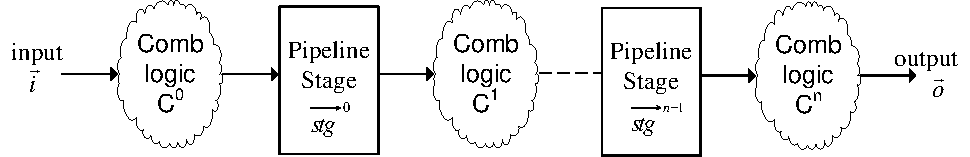
\includegraphics[width=0.5\textwidth]{pipemod_pipeline}
\end{center}
\caption{编码器的一般性结构}
  \label{fig_pipeenc}
\end{figure}


因此,
每个$C^j$ 可以视为一个小型的编码器用于从$\vec{stg}^{j-1}$或$\vec{i}$中计算$\vec{stg}^j$ 或$\vec{o}$。


在本文的剩余部分,
上标始终表示特定的流水线级,,
而下标则如小节\ref{subsec_fsm}所述,
表示在展开的迁移关系序列中的步数。
例如,
$\vec{stg}^j$ 是第$j$个流水线级。
而$\vec{stg}^j_i$ 则是该第$j$流水线级
在展开的迁移函数序列中的第$i$步的值。

\subsection{推导$p$, $l$ 和$r$}\label{subsec_inferplr}
在推导之前,
我们首先使用算法\ref{alg_pcln} 以得到$p$, $l$ 和$r$ 。

因为存在多于一个$i\in \vec{i}$,
我们需要为每一个$i\in \vec{i}$使用算法\ref{alg_pcln}
以得到他们对用的$p$, $l$ 和$r$ 。

然后我们将最终的$p$,$l$ 和$r$ 设置为所有$i\in \vec{i}$中最大的$p$, $l$ 和$r$ 。
根据公式\ref{uniqt1},
这些$p$, $l$ 和$r$ 能够使得$<o_{p},\dots,o_{p+l+r}>$ 唯一决定所有$i_{p+l}\in \vec{i}_{p+l}$。


\subsection{压缩$r$ 和$l$}\label{reduceing}

\begin{algorithm}[t]
\begin{algorithmic}[1]
\FOR{$r':=r \to 0$}
\label{testr_1}
  \IF{$r'\equiv 0$ or $F_{PC}(p,l,r'-1)$ 对于某些$i\in \vec{i}$是可满足的}
  \STATE  break;
  \ENDIF
\ENDFOR
\RETURN $r'$;
\caption{$RemoveRedundancy(p,l,r)$}
\label{algo_remove2}
\end{algorithmic}
\end{algorithm}



算法\ref{alg_pcln} 同步增长$p$, $l$ 和$r$ ,
因此在$l$ 和$r$中可能存在冗余。
因此我们需要首先在算法\ref{algo_remove2}中压缩$r$。


在行\ref{testr_1},
当$F_{PC}(p,l,r'-1)$ 可满足时,
则$r'$ 是最有一个使得$F_{PC}(p,l,r')$ 不可满足的,
我们将其直接返回。
另一方面,
当$r'\equiv 0$,
$F_{PC}(p,l,0)$ 已经在上一次迭代中被测试过,
且结果必然是不可满足。
在这种情况下我们返回$0$。


如此,
我们从算法\ref{algo_remove2}获得了一个压缩后的$r$ ,
它能使$\vec{i}_{p+l}$ 被$<\vec{o}_{p},\dots,\vec{o}_{p+l+r}>$唯一决定。

我们进一步要求:
\begin{enumerate}
 \item 如图\ref{fig_pc1}所示,
 $l$ 可以被压缩为0,
 这意味着$\vec{i}_{p}$ 能够被$<\vec{o}_{p},\dots,\vec{o}_{p+r}>$唯一决定,
 也就是说,
 所有的将来输出。
 \item 上述的序列$<\vec{o}_{p},\dots,\vec{o}_{p+r}>$
 可以被进一步压缩为$\vec{o}_{p+r}$.
 这意味着$\vec{o}_{p+r}$ 是在恢复$\vec{i}_p$时唯一被需要的输出。
\end{enumerate}

检查上述两个要求等价于下式的不可满足:

\begin{multline}\label{uniqt11}
% \begin{split}
F'_{PC}(p,r):=\\
\left\{
\begin{array}{cc}
&\bigwedge_{m=0}^{p+r}
\{
(\vec{s}_{m+1},\vec{o}_m)\equiv T(\vec{s}_m,\vec{i}_m)
\}
\\
\wedge&\bigwedge_{m=0}^{p+r}
\{
(\vec{s'}_{m+1},\vec{o'}_m)\equiv T(\vec{s'}_m,\vec{i'}_m)
\}
\\
\wedge&\vec{o}_{p+r}\equiv \vec{o'}_{p+r} \\
\wedge& i_{p}\equiv 1 \wedge  i'_{p}\equiv 0
% \wedge&\bigwedge_{m=0}^{p+l+r}assertion(\vec{i}_m) \\
% \wedge&\bigwedge_{m=0}^{p+l+r}assertion(\vec{i'}_m)
\end{array}
\right\}
% \end{split}
\end{multline}


该等式看起来似乎远强于等式(\ref{uniqt1})。
我们将在实验结果中指出,
该等式总能称为不满足。

\begin{figure}[t]
\begin{center}
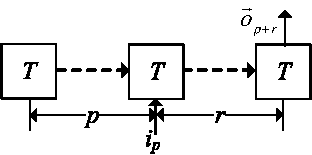
\includegraphics[width=0.25\textwidth]{pc1}
\end{center}
\caption{从压缩的输出序列中恢复输入}
  \label{fig_pc1}
\end{figure}

\subsection{推导流水线}\label{subsec_inferstage}

基于上述的$p$ 和$r$,
我们将上述公式(\ref{uniqt11})中的$F'_{PC}$ 推广到下述公式
以便能够检查 $v$在第$j$步
是否能够被$\vec{w}$ 在第$k$步唯一决定。
现在$v$ 和$\vec{w}$ 可以使输入,输出和状态变量向量。

\begin{multline}\label{uniqt2}
% \begin{split}
F''_{PC}(p,r,v,j,\vec{w},k):=\\
\left\{
\begin{array}{cc}
&\bigwedge_{m=0}^{p+r}
\{
(\vec{s}_{m+1},\vec{o}_m)\equiv T(\vec{s}_m,\vec{i}_m)
\}
\\
\wedge&\bigwedge_{m=0}^{p+r}
\{
(\vec{s'}_{m+1},\vec{o'}_m)\equiv T(\vec{s'}_m,\vec{i'}_m)
\}
\\
\wedge&\vec{w}_{k}\equiv \vec{w'}_{k} \\
\wedge& v_{j}\equiv 1 \wedge  v'_{j}\equiv 0
% \wedge&\bigwedge_{m=0}^{p+l+r}assertion(\vec{i}_m) \\
% \wedge&\bigwedge_{m=0}^{p+l+r}assertion(\vec{i'}_m)
\end{array}
\right\}
% \end{split}
\end{multline}

很显然,
当$F''_{PC}(p,r,v,j,\vec{w},k)$ 不可满足时,
$\vec{w}_k$ 能够唯一决定$v_j$.

最后一集流水线$\vec{stg}^{n-1}$ 就是
所有能够被
在第$p+r$步的$\vec{o}$唯一决定的$s\in \vec{s}$。
其定义为:

\begin{multline}\label{stgn_1}
 \vec{stg}^{n-1} :=
\left\{
 s\in \vec{s} ~|
\begin{array}{cc}
 F''_{PC}(p,r,
 s,p+r,
 \vec{o},p+r)\\
 ~is~unsatisfiable
\end{array}
\right\}
\end{multline}


类似的,
对于$0\le j\le n-2$,
$\vec{stg}^j$ 在第$j-((n-2)-(p+r-1))$步
可以被$\vec{stg}^{j+1}$ 在第$j-((n-2)-(p+r-1))+1$步唯一决定。
我们可以定义$\vec{stg}^j$ 为:

\begin{multline}\label{stgn_def}
\begin{array}{ccc}
S             & := & \vec{s}/\bigcup_{j<k\le n-2}\vec{stg}^{k}\\
D             & := & (n-2)-(p+r-1)\\
\end{array}
\end{multline}

\begin{multline}\label{stgn_j}
\vec{stg}^{j} := \\
 \left\{
 s\in S ~|
\begin{array}{cc}
 F''_{PC}(p,r,s,j-D,\vec{stg}^{j+1},j-D+1)\\
不可满足
\end{array}
\right\}
\end{multline}

基于等式(\ref{stgn_1}) 和(\ref{stgn_j}),
所有的流水线几都能够被推导出来。

\subsection{推导唯一决定输入的流水线级}\label{subsec_inferinput}

根据图\ref{fig_pipeenc},
 定义于(\ref{stgn_j}) 的$\vec{stg}^0$是唯一决定$\vec{i}$的流水线级。

然而在实际的解码器中,
并不一定是这种情形。
因此我们需要从$0$ 到$n-1$,
搜索最小的$j$ 使得
$\vec{i}$ 能够被$\vec{stg}^j$唯一决定。
即,
最小的能够使得$F''_{PC}(p,r,i,p,\vec{stg}^{j},j-D)$ 对所有$i\in \vec{i}$不可满足的$j$。
其中$D$ 定义于等式(\ref{stgn_def})。

\section{特征化输入向量和流水线级的布尔函数}\label{sec_char}
\subsection{特征化最后一个流水线级的布尔函数}

根据等式(\ref{stgn_1}),
每个寄存器$s\in \vec{stg}^{n-1}$ 都能够被$\vec{o}$ 在第$p+r$步唯一决定。
即,
$F''_{PC}(p,r,s,p+r,\vec{o},p+r)$ 不可满足,且可以被划分为:

\begin{multline}
 \phi_A := \\
 \left\{
\begin{array}{cc}
&\bigwedge_{m=0}^{p+r}
\{
(\vec{s}_{m+1},\vec{o}_m)\equiv T(\vec{s}_m,\vec{i}_m)
\}
\\
\wedge& s_{p+r}\equiv 1
\end{array}
\right\}
\end{multline}

\begin{multline}
% \begin{split}
\phi_B := \\
\left\{
\begin{array}{cc}
&\bigwedge_{m=0}^{p+r}
\{
(\vec{s'}_{m+1},\vec{o'}_m)\equiv T(\vec{s'}_m,\vec{i'}_m)
\}
\\
\wedge&\vec{o}_{p+r}\equiv \vec{o'}_{p+r} \\
\wedge& s'_{p+r}\equiv 0
% \wedge&\bigwedge_{m=0}^{p+l+r}assertion(\vec{i}_m) \\
% \wedge&\bigwedge_{m=0}^{p+l+r}assertion(\vec{i'}_m)
\end{array}
\right\}
% \end{split}
\end{multline}

由于$F''_{PC}(p,r,s,p+r,\vec{o},p+r)$ 等价于$\phi_A \wedge \phi_B$,
因此$\phi_A \wedge \phi_B$ 也是不可满足的。
而$\phi_A$ 和$\phi_B$ 的共同变量集合是$\vec{o}_{p+r}$。

根据\cite{InterpBoolFunction},
$\phi_A$ 相对于$\phi_B$的Craig插值$\phi_I$  可以构造出来,
其中仅包含$\vec{o}_{p+r}$,
并覆盖所有使$s_{p+r}\equiv 1$得$\vec{o}_{p+r}$ 的赋值。
同时,
$\phi_I\wedge \phi_B$  不可满足,
这意味着$\phi_I$ 不能使$s_{p+r}\equiv 0$。

因此,
$\phi_I$ 能作为解码器的布尔函数以从$\vec{o}$中恢复$s\in \vec{stg}^{n-1}$ 。

\subsection{特征化其他流水线级的布尔函数}
类似于上一小节,
我们可以将公式(\ref{stgn_j})中的不可满足公式$F''_{PC}(p,r,s,j-D,\vec{stg}^{j+1},j-D+1)$
划分如下:

\begin{multline}
 \phi_A := \\
 \left\{
\begin{array}{cc}
&\bigwedge_{m=0}^{p+r}
\{
(\vec{s}_{m+1},\vec{o}_m)\equiv T(\vec{s}_m,\vec{i}_m)
\}
\\
\wedge& s_{j-D}\equiv 1
\end{array}
\right\}
\end{multline}

\begin{multline}
% \begin{split}
\phi_B := \\
\left\{
\begin{array}{cc}
&\bigwedge_{m=0}^{p+r}
\{
(\vec{s'}_{m+1},\vec{o'}_m)\equiv T(\vec{s'}_m,\vec{i'}_m)
\}
\\
\wedge&\vec{stg}^{j+1}_{j-D+1}\equiv \vec{stg'}^{j+1}_{j-D+1} \\
\wedge& s'_{j-D}\equiv 0
% \wedge&\bigwedge_{m=0}^{p+l+r}assertion(\vec{i}_m) \\
% \wedge&\bigwedge_{m=0}^{p+l+r}assertion(\vec{i'}_m)
\end{array}
\right\}
% \end{split}
\end{multline}

$\phi_A$ 相对于$\phi_B$的Craig 插值$\phi_I$  能够被构造出来,
并作为从$\vec{stg}^{j+1}$恢复$s\in \vec{stg}^{j}$的布尔函数。

\subsection{特征化输入变量的布尔函数}

根据小节\ref{sec_pipeinfer},
我们找到了使得$F''_{PC}(p,r,i,p,\vec{stg}^{j},j-D)$ 对所有$i\in \vec{i}$都不满足的$j$,
其中$D$ 在的公式(\ref{stgn_def})中定义。
$F''_{PC}(p,r,i,p,\vec{stg}^{j},j-D)$ 是不可满足的并可划分为:

\begin{multline}
% \begin{split}
\phi_A:=\\
\left\{
\begin{array}{cc}
&\bigwedge_{m=0}^{p+r}
\{
(\vec{s}_{m+1},\vec{o}_m)\equiv T(\vec{s}_m,\vec{i}_m)
\}
\\
\wedge& i_{p}\equiv 1
% \wedge&\bigwedge_{m=0}^{p+l+r}assertion(\vec{i}_m) \\
% \wedge&\bigwedge_{m=0}^{p+l+r}assertion(\vec{i'}_m)
\end{array}
\right\}
% \end{split}
\end{multline}

\begin{multline}
% \begin{split}
\phi_B:=\\
\left\{
\begin{array}{cc}
&\bigwedge_{m=0}^{p+r}
\{
(\vec{s'}_{m+1},\vec{o'}_m)\equiv T(\vec{s'}_m,\vec{i'}_m)
\}
\\
\wedge&\vec{stg}^j_{j-D}\equiv \vec{stg'}^j_{j-D} \\
\wedge& i'_{p}\equiv 0
% \wedge&\bigwedge_{m=0}^{p+l+r}assertion(\vec{i}_m) \\
% \wedge&\bigwedge_{m=0}^{p+l+r}assertion(\vec{i'}_m)
\end{array}
\right\}
% \end{split}
\end{multline}

和上一小节类似,
$\phi_A$ 相对于$\phi_B$的Craig 插值$\phi_I$
可以作为从$\vec{stg}^j$中恢复$i\in\vec{i}$的布尔函数。



\section{实验结果}\label{sec_exp}
我们在OCaml 语言中实现了上述算法,
并使用MiniSat 1.14 \cite{EXTSAT}求解相应的公式。
使用一台包含16 个Intel Xeon E5648 2.67GHz处理器,
192GB 存储器, 和CentOS 5.4 Linux操作系统的服务器。

表\ref{tab_bench} 给出了本文使用的benchmarks 。
第2和3列分别给出了每个benchmark的输入, 输出和寄存器数量。
第4列将这些编码器映射至LSI10K 库的面积。
本文中,
所有的面积和延时都是在相同的设定下得到的。



\begin{table*}[t]
\caption{Benchmarks and experimental results}
\begin{tabular}{|c|c|c|c|c|c|c|c|c|c|c|c|}
\hline
 Names     & \multicolumn{4}{|c|}{编码器}                                  &   \multicolumn{3}{|c|}{由\cite{ShenTCAD11}产生}             &   \multicolumn{4}{|c|}{本文产生} \\
           & \multicolumn{4}{|c|}{}                                              &   \multicolumn{3}{|c|}{的解码器}  &   \multicolumn{4}{|c|}{的解码器} \\\cline{2-12}
           &    \#   &   \#    &面积& 编码器&运行&延迟&面积                                       &运行&延迟&面积&寄存器\\
           & in/out  &  reg    &      &   描述&时间&(ns) &                                        &时间 &(ns) &    &个数\\\hline\hline
 pcie      & 10/11   & 23      & 326  &PCIE 2.0 \cite{pcie21}                    &0.37 &7.20 &624                                     &3.57 & 5.89&652 &9/12\\\hline
 xgxs      & 10/10   & 16      & 453  &     以太网clause 48 \cite{IEEE8023_S4}&0.21 &7.02 &540                                     &1.57 & 5.93&829 &13\\\hline
 t2eth     & 14/14   & 49      & 2252 &    以太网clause 36 \cite{IEEE8023_S4} &12.7 &6.54 &434                                     &47.2 & 6.12&877 &8/8/10/20\\\hline
scrambler  &64/64    & 58      & 1034 & inserting 01 flipping                    &     \multicolumn{7}{|c|}{no pipeline }\\\cline{1-5}
 xfi       & 72/66   & 72      & 7772 &     以太网clause 49 \cite{IEEE8023_S4}&     \multicolumn{7}{|c|}{stages found}\\\hline
\end{tabular}\label{tab_bench}
\end{table*}





第6到8列分别给出了\cite{ShenTCAD11}算法在产生误流水线的解码器时的运行时间,延迟和面积。
而第9到11列分别给出了本文算法的运行时间,延迟和面积。
而最后一列给出了每一级流水线包含的寄存器个数。

比较第7和10列可以看到
解码器的延迟得到了较大的改善,
而最后一列指出确实存在很深的流水线,
其中t2ether包含4级流水线。

有一点非常有意思的是,
两个最大的benchmarks scrambler 和xfi 没有检测到流水线。
我们研究了其代码,并确认了这一点。
他们的面积如此之大是因为使用了64 到72 位宽的数据路径。

\section{相关工作}\label{sec_relwork}
沈等\cite{ShenICCAD09} 提出了第一个对偶综合算法。
他通过迭代的展开迁移函数来检测解码器的存在性。
并通过遍历可满足赋值了产生解码器函数。
但是该算法是不停机的,并且在产生解码器时非常慢。

沈 et al.\cite{ShenTCAD11} 和刘at al.\cite{LiuICCAD11} 分别独立处理了停机问题,
方法是在状态序列中检测环形路径。
而解码器构造中运行时间太长的问题则在\cite{ShenTCAD12,LiuICCAD11} 中通过Craig插值\cite{InterpBoolFunction}解决。

沈et al. \cite{ShenTCAD12} 推导了能够使得解码器存在的配置断言。

屠et al.\cite{TuDAC13} 提出了一个突破性的算法能够在构造解码器时考虑整个无限的输入历史。

% This algorithm can handle some encoders that cannot be handled by the state-of-the-art algorithms.
% Their work is orthogonal to ours.

% \subsection{Program inversion}\label{subsec_proinv}
% % According to \cite{dim_syn},
% Program inversion derives a program $P^{-1}$
% that negates the computation of a given program $P$.
% So
% it is very similar to complementary synthesis.
%
% The initial work on program inversion \cite{prog_inv} used proof-based approaches,
% which could handle only very small programs and very simple syntax structures.
%
% \cite{mtd_autoProginv} inverted first-order functional programs
% by eliminating nondeterminism with LR-based parsing methods.
% But
% the use of functional languages in that work is incompatible with our complementary synthesis.
%
% \cite{program_inversion_11} assumed that an inverse program was related to the original program,
% so the space of possible inversions can be inferred by automatically
% mining the original program for expressions, predicates, and control flow.
% This algorithm inductively rules out invalid paths that can't fulfill the requirement of inversion
% % to narrow down the space of candidate programs
% until only the valid ones remain.
% So,
% it can't guarantee the correctness of its solution if its assumptions don't hold.

% \subsection{The completeness of bounded model checking}\label{subsec_bmc_relate}
% Bounded model checking(BMC) \cite{bmc_tacas99} is a model checking technology that considers only paths of limited length.
% So it is an incomplete algorithm.
% Many researchers have tried to find complete approaches for BMC.
%
% One line of research\cite{bmc_tacas99,RecDiam} tried to find out a bound $b$,
% which can guarantee the correctness of a specification,
% if the specification is correct on all paths that are shorter than $b$.
% Line 8 of Algorithm \ref{algo_infer} finds out the value of $p$,$d$ and $l$ that can prove the non-existence of the decoder,
% which is similar to \cite{bmc_tacas99,RecDiam}.
%
% The other line of research\cite{kind_tacas99} tried to find a bound for induction,
% such that the correctness of a specification within any bound $b$ implies the correctness on bound $b+1$.
% Our algorithm proves the non-existence of the decoder by unfolding loops.
% This is similar to finding induction patterns \cite{kind_tacas99}.

% \textbf{This paper achieves completeness without following these two approaches.
% Instead,
% it defines two complement uniqueness conditions,
% $LP$ and $LL$,
% and find out proper algorithms to check them.}

%\subsection{Temporal Logic Synthesis}
%%Automatically synthesis of program from logic specification is first identified as Church's problem in 1962\cite{LOGARTHAUTO}.
%%Some early researches \cite{SLVSQFSS,AUTOINF} solve this problem by reducing it to checking emptiness of tree automata.
%
%The temporal logic synthesis was first addressed by Clarke et al.\cite{DSGSYNTMPLG} and Manna et al. \cite{SYNTMPLGSPC}.
%But Pnueli et al. \cite{SYNRCTVMD} pointed out that the complexity of LTL synthesis is double exponent.
%%This high complexity drives researchers turning their focus to find smaller but still useful subset of temporal logic,
%%such that synthesis problem can be solved with lower complexity.
%
%One line of research \cite{CNTLSYNTMDAUTO,DTMGENGMELTL,SYNRCTVDES} focuses on the so-called generalized reactive formulas of the form:
%$(\square \lozenge p_1 \wedge \cdots \square \lozenge p_m) \to (\square \lozenge q_1 \wedge \cdots \square \lozenge q_n)$.
%Complexity of solving synthesis problem for such formula is $O(N^3)$.
%
%The other line of research focuses on finding efficient algorithm \cite{SYNCNTLBNDRPN}
%for expensive safra determination algorithm \cite{CMPLXAUTO} on an useful formula subset,
%or just avoiding it\cite{NEWALGSTRGSYN}.
%
%%Yet another approach is antichain\cite{ANTICHAIN},
%%which reduces the expensive state set computation to computation on maximal and minimal elements of lattice.
%
%Based on these research works,
%some tools\cite{ANZU} that can handle small temporal formulas have been developed.
%
%All these works assume a hostile environment,
%which seems too restrictive for many applications.
%So Fisman et al. \cite{rationalsyn_tacas10}, Chatterjee et al. \cite{assguasyn_tacas07} and Ummels et al. \cite{ralgame_istta06} proposed rational synthesis algorithm,
%which assumes that each agents act to achieve their own goals instead of failing each other.


% \subsection{Protocol converter synthesis}
% Protocol converter synthesis is a process that automatically generates a translator between two different communication protocols.
% This is relevant to our work,
% because both focus on synthesizing communication circuits.
%
% In \cite{converter_date08,converter_todeas09},
% Avnit et al. first defined a general model for describing different protocols,
% and then provided an algorithm to decide
% whether there is some functionality of a protocol that cannot be translated into another.
% Finally,
% they synthesized a translator by computing the greatest fixed point for the update function of the buffer's control states.
% Latter in \cite{converter_date09},
% they improved their algorithm with a more efficient design space exploration algorithm.

% \subsection{Satisfying Assignments Enumeration}\label{subsec_relallsat}
%
% Some algorithms try to enumerate all satisfying assignments faster
% by enlarging each complete satisfying assignment.
% % so that a large state set that contains more complete satisfying assignments can be obtained.
% \cite{SATUNBMC} constructs an alternative implication graph in SAT solver,
% which records the reasoning relation that leads to the assignment of a particular variable.
% All variables outside this graph can be ruled out from the complete assignment.
% In \cite{MINASS} and \cite{REPARAM},
% those variables whose absence can't make $obj\equiv 0$ satisfiable are removed one by one.
% In \cite{MINCEX} and \cite{PRIMECLAUSE},
% conflict analysis based approaches are used
% to remove multiple irrelevant variables in one SAT run.
% In \cite{MEMEFFALLSAT},
% the variable set is divided into an important subset and an unimportant subset.
% Variables in the important subset have higher decision priority than those unimportant ones.
% Thus,
% the important subset forms a search tree,
% with each leaf being another search tree for the unimportant set.
% %Tobias Nopper et al.\cite{CMPMINCEX} propose an counterexample minimization algorithm for incomplete designs that contain black box.
% \cite{EFFSATUSMCCO} qualifies out unimportant variables by setting them to constant value returned by the SAT solver.
%
% Other algorithms constructs interpolations to cover more satisfying assignments.
% \cite{InterpBoolFunction}
% constructs a first formula that contradicts with another formula,
% from which an interpolation can be derived and used as an over-approximation of the first formula.
% \cite{interpNoProof} generates
% interpolation with a framework similar to the iterative enumerating and
% enlarging approaches mentioned above.
% But there are two enlarging steps for each enumerated assignment,
% in which the assignments are enlarged with respect to the two formulas involved in constructing interpolant.
% It is the first paper that constructs interpolant without proof.

% \subsection{Logic synthesis with Craig interpolation}
% In \cite{scalableFuncDep,Bidecomp},
% the functional dependency and logic decomposition problems are solved
% by formulating the base Boolean functions' output bits as the input bits to an unknown Boolean function,
% and characterize this unknown function by Craig interpolation.
% This algorithm is also used in our paper \cite{ShenTCAD12} to find out all the possible decoders.
%
% % In \cite{ecoInterp},
% % an ECO is generated with Craig interpolation.
%
% In \cite{InterpBoolFunction},
% the first algorithm to characterize a Boolean function from a Boolean Relation was proposed.
% It includes two different algorithms:
% The first one handle a general  non-deterministic Boolean relation that can't uniquely determined its output,
% The second one is a special case of the first one
% that handles a deterministic relation that can uniquely determine its output by Craig interpolation.
% The second one is used in \cite{ShenTCAD12}.
%
% This paper also need to handle a non-deterministic Boolean relation,
% which seems to be similar to that one handled by the first algorithm of \cite{InterpBoolFunction}.
% But our case is much more complicated,
% because the Boolean relation to be handled is an unrolled transition function with unknown length.
% That is,
% we must first find out the value of $p$, $l$ and $r$.
% But these value must be determine together with finding out the flow control vector $\vec{f}$.
% So the way we handle non-determinism is significantly different from that of \cite{InterpBoolFunction}.
% But after we got the value of $p$, $l$ and $r$,
% together with the flow control vector $\vec{f}$ and the predicate $valid(\vec{f})$,
% we can characterize the decoder's Boolean function with an algorithm similar to the second one in \cite{InterpBoolFunction}.

\section{结论}\label{sec_conclude}

本文提出了第一个能够处理流水线的对偶综合算法。
实验结果表明,
本算法能够针对多个复杂的实际工业界编码器,
正确的推导流水线结构并生成对应的流水线解码器。.



